\documentclass[conference]{IEEEtran}
\IEEEoverridecommandlockouts

\usepackage{cite}
\usepackage{amsmath,amssymb,amsfonts}
\usepackage{algorithmic}
\usepackage{graphicx}
\usepackage{textcomp}
\usepackage{xcolor}
\usepackage{booktabs}
\usepackage{url}
\usepackage[hidelinks]{hyperref}
\usepackage{caption}

\bibliographystyle{IEEEtran}

\graphicspath{{figures/}}

% Numbers, tables and figures are generated from results/*.json by
% scripts/make_report_tables.py and scripts/make_figures.py. Nothing numeric in
% this document is typed by hand.
% Generated by scripts/make_report_tables.py -- do not edit by hand.

\newcommand{\BestModelLabel}{BPMF}
\newcommand{\BestRMSE}{0.9087}
\newcommand{\BestRMSECI}{0.0050}
\newcommand{\NumSeeds}{5}
\newcommand{\GlobalMeanRMSE}{1.1225}
\newcommand{\GlobalMeanRMSECI}{0.0044}
\newcommand{\ItemMeanRMSE}{1.0247}
\newcommand{\ItemMeanRMSECI}{0.0036}
\newcommand{\UserMeanRMSE}{1.0402}
\newcommand{\UserMeanRMSECI}{0.0065}
\newcommand{\BiasBaselineRMSE}{0.9428}
\newcommand{\BiasBaselineRMSECI}{0.0046}
\newcommand{\PMFRMSE}{0.9311}
\newcommand{\PMFRMSECI}{0.0046}
\newcommand{\PMFBiasRMSE}{0.9144}
\newcommand{\PMFBiasRMSECI}{0.0053}
\newcommand{\PMFLogisticRMSE}{0.9272}
\newcommand{\PMFLogisticRMSECI}{0.0039}
\newcommand{\BPMFRMSE}{0.9087}
\newcommand{\BPMFRMSECI}{0.0050}
\newcommand{\BestRMSEOneM}{0.8644}
\newcommand{\BestModelLabelOneM}{PMF + biases}
\newcommand{\LegacyRMSE}{0.9669}
\newcommand{\LegacyRMSEStd}{0.0061}
\newcommand{\LegacyRMSEMin}{0.9571}
\newcommand{\LegacyRMSEMax}{0.9724}
\newcommand{\LegacyReportedTrain}{0.8968}
\newcommand{\LegacyTrueTrain}{0.8963}
\newcommand{\LegacyPenaltyInflation}{0.0005}
\newcommand{\LegacySeeds}{5}
\newcommand{\ScalingSlope}{1.151}
\newcommand{\ScalingSlopeLow}{1.068}
\newcommand{\ScalingSlopeHigh}{1.234}
\newcommand{\ScalingRSquared}{0.989}
\newcommand{\ScalingSupported}{yes}
\newcommand{\ScalingMaxN}{800,167}
\newcommand{\ScalingMinN}{7,983}
\newcommand{\ScalingSlopeOneHundredK}{0.976~[0.951, 1.001]}
\newcommand{\ScalingSlopeOneM}{0.994~[0.983, 1.005]}
\newcommand{\NumClaims}{3}
\newcommand{\ClaimedRMSE}{1.0109}
\newcommand{\ClaimVerdict}{partially supported}
\newcommand{\ClaimConfigsTried}{48}
\newcommand{\ClaimConfigsBetter}{34}
\newcommand{\ClaimBestReachable}{0.9354}
\newcommand{\LogisticGain}{0.0047}
\newcommand{\ClipGain}{0.0000}
\newcommand{\IdentityOutOfRangePct}{0.08}
\newcommand{\BestLatentDim}{20}
\newcommand{\BestLatentRMSE}{0.9334}
\newcommand{\BestLambda}{0.1}
\newcommand{\BestLambdaRMSE}{0.9414}
\newcommand{\NoRegCost}{0.2240}
\newcommand{\NUsersOneHundredK}{943}
\newcommand{\NItemsOneHundredK}{1,682}
\newcommand{\NRatingsOneHundredK}{100,000}
\newcommand{\DensityOneHundredK}{6.30}
\newcommand{\NUsersOneM}{6,040}
\newcommand{\NItemsOneM}{3,706}
\newcommand{\NRatingsOneM}{1,000,209}
\newcommand{\DensityOneM}{4.47}


\def\BibTeX{{\rm B\kern-.05em{\sc i\kern-.025em b}\kern-.08em
    T\kern-.1667em\lower.7ex\hbox{E}\kern-.125emX}}

\begin{document}

\title{Probabilistic and Bayesian Matrix Factorization\\
for Recommender Systems: A Comparative Study on MovieLens}

\author{\IEEEauthorblockN{Nkosenhle Ndlovu}
\IEEEauthorblockA{\textit{School of Computer Science and Applied Mathematics} \\
\textit{University of the Witwatersrand, Johannesburg}\\
Johannesburg, South Africa \\
2539199@students.wits.ac.za}
}

\maketitle

\begin{abstract}
Recommendation systems reduce information overload by selecting items for a user from
interaction history or from similarity in taste, and collaborative filtering (CF) is the
dominant family of methods for doing so. Much of the work within CF rests on matrix
factorization (MF). This paper reports a controlled comparison of five factorization
models --- maximum a posteriori Probabilistic Matrix Factorization (PMF), PMF with additive
biases, PMF under a logistic link, PMF trained with Adam, and Bayesian PMF (BPMF) with
Gibbs sampling --- against four non-factorization baselines, on MovieLens 100K and 1M over
repeated random splits with confidence intervals. Four results follow. BPMF is the
strongest model at \BestRMSE, and its advantage over MAP estimation concentrates in
low-activity users rather than spreading evenly. A closed-form additive bias model reaches
\BiasBaselineRMSE{} with no interaction term at all, so most of the achievable accuracy on
this data is additive and the increment attributable to latent structure, while real, is
the smaller quantity. Regularization strength is the largest single hyperparameter effect;
latent dimensionality matters considerably less once early stopping is present, since early
stopping is itself performing capacity control. Finally, training cost is linear in the
number of observations at fixed model size, with within-dataset log--log exponents of
\ScalingSlopeOneHundredK{} and \ScalingSlopeOneM, while a pooled fit across datasets is
inflated to \ScalingSlope{} by the dense momentum update rather than by any superlinearity
in the algorithm. All code, data preparation and results are released, and every number
reported here is regenerated from stored experiment output rather than transcribed.
\end{abstract}

\begin{IEEEkeywords}
Recommendation systems, collaborative filtering, probabilistic matrix factorization,
Bayesian inference, reproducibility
\end{IEEEkeywords}

\section{Introduction}

Recommendation methods are classified largely into two fields: content-based methods and
collaborative filtering (CF) methods \cite{liu2013bayesian}. In content-based
recommendation, the rating of an item for a given user is estimated from the ratings of
similar items the user has already interacted with.

CF is widely used because it works. Its underlying assumptions are that an active user's
past interactions are indicative of that user's preferences, and that similar users have
similar tastes. Matrix Factorization (MF) is a CF-type model and has proven an effective
model-based method \cite{koren2009matrix}, resting on the assumption that the user--item
relationship $R$ is explained by a small number of latent features $U$ and $V$ with
\[R \approx U^\top V.\]

This notion is familiar from linear algebra, and many early MF recommenders used
deterministic techniques such as Singular Value Decomposition (SVD). Two difficulties
follow them. \emph{Data sparsity}: for a large dataset, $R$ contains overwhelmingly many
missing values, because not every user records a rating for every item they encounter.
Since MF methods link users by identifying linear dependencies among rows of $R$,
sparseness makes that overlay difficult and the results unstable. \emph{Cold start}: for a
new user there is no interaction history at all, and MF-based recommenders predict badly.
Mnih and Salakhutdinov \cite{mnih2007probabilistic} additionally argue that such models do
not scale to very large datasets.

Probabilistic factor-based models address this by treating the hidden factors as random
variables with directed connections to the observed ratings
\cite{mnih2007probabilistic}. PMF computes point estimates of the posterior over those
factors; its training scales linearly with the number of observations and it performs well
on sparse, imbalanced data such as the Netflix corpus \cite{bennett2007netflix}. The
drawback is inherited from Bayesian modelling generally: exact inference is intractable,
and MAP estimation requires the prior variances to be fixed by hand.

Salakhutdinov and Mnih later proposed Bayesian PMF (BPMF) \cite{salakhutdinov2008bayesian},
which places Gaussian--Wishart hyperpriors on the factor priors and integrates over them by
Markov chain Monte Carlo, removing the manual regularisation tuning. Separately, Liu
\emph{et al.}\ \cite{liu2013bayesian} extended BPMF by fusing social relations and item
contents, arguing that BPMF's hyperparameters are shared across all users whereas in
practice user preferences vary greatly; related probabilistic treatments of social
information include SoRec \cite{ma2008sorec}. The main shortcoming of PMF that these works
address is that careful parameter tuning is required to avoid overfitting.

\subsection{Scope and contributions}

The literature reports PMF and BPMF results principally on the Netflix corpus, at a scale
where the capacity/data balance differs sharply from the benchmarks most practitioners
work with. It also reports them largely without the non-factorisation baselines against
which an RMSE becomes interpretable --- an omission that has been shown to reverse
published conclusions when corrected \cite{rendle2019difficulty}, and to account for a
substantial fraction of improvements that do not survive re-evaluation
\cite{dacrema2019worrying}. This paper measures the family on MovieLens under a single
protocol, with those baselines present throughout. Its contributions are:

\begin{itemize}
  \item a from-scratch implementation of PMF, biased PMF, a logistic-link variant, an
        Adam-trained variant, and BPMF by Gibbs sampling, with analytic gradients verified
        against central finite differences for every variant;
  \item a controlled comparison against four non-factorisation baselines over \NumSeeds{}
        random splits with confidence intervals, on MovieLens 100K and 1M;
  \item ablations isolating the contribution of latent dimensionality, regularisation
        strength, link function and optimiser, with early stopping treated as the
        capacity-control mechanism it is;
  \item test error stratified by user activity, locating where the Bayesian treatment's
        advantage actually arises; and
  \item a direct measurement of how training cost scales in the number of observations,
        separating the algorithm's complexity from the optimiser's bookkeeping.
\end{itemize}

\section{PMF Design}
\label{section:pmf-design}

Let $R \in \mathbb{R}^{n \times m}$ denote a user--item rating matrix, where $n$ is the
number of users and $m$ the number of items. Each entry $R_{ij}$ is the rating that user
$i$ assigns to item $j$, taking values in a discrete range $[1,k]$ with $k \in \mathbb{Z}$.
Because of sparsity, most entries are unobserved.

Define two low-rank latent matrices, the user feature matrix $U \in \mathbb{R}^{d\times n}$
and the item feature matrix $V \in \mathbb{R}^{d \times m}$, whose columns $\mathbf{u}_i
\in \mathbb{R}^d$ and $\mathbf{v}_j \in \mathbb{R}^d$ are the latent feature vectors of user
$i$ and item $j$. These capture the preferences and attributes that govern the ratings.

The key assumption of PMF is that observed ratings are noisy inner products of the user and
item features. The \emph{likelihood} of the observed ratings is therefore Gaussian with
mean $\mathbf{u}_i^\top\mathbf{v}_j$ and a global noise variance $\sigma^2$:

\begin{equation}
  p(R \mid U, V, \sigma^2) =
    \prod_{i=1}^{n}\prod_{j=1}^{m}
    \left[\mathcal{N}\!\left(R_{ij} \mid \mathbf{u}_i^\top\mathbf{v}_j, \sigma^2\right)\right]^{I_{ij}}
  \label{eq:likelihood}
\end{equation}

where $\mathcal{N}(x \mid \mu,\sigma^2)$ is the Gaussian density and $I_{ij}$ is an
indicator equal to $1$ when $R_{ij}$ is observed. Equation \eqref{eq:likelihood} is the
likelihood; the posterior follows only after multiplying by the priors in
\eqref{eq:priors}.

To regularise the model we impose zero-mean spherical Gaussian priors on the features:
\begin{equation}
\begin{aligned}
  p(U \mid \sigma_U^2) &= \prod_{i=1}^{n}\mathcal{N}(\mathbf{u}_i \mid \mathbf{0}, \sigma_U^2\mathbf{I}),\\
  p(V \mid \sigma_V^2) &= \prod_{j=1}^{m}\mathcal{N}(\mathbf{v}_j \mid \mathbf{0}, \sigma_V^2\mathbf{I}).
\end{aligned}
\label{eq:priors}
\end{equation}

Maximising the log posterior with respect to $U$ and $V$, with the hyperparameters held
fixed, is equivalent to minimising the regularised squared error

\begin{equation}
\begin{split}
  E &= \frac{1}{2}\sum_{i=1}^{n}\sum_{j=1}^{m} I_{ij}\left(R_{ij} - \mathbf{u}_i^\top\mathbf{v}_j\right)^2\\
    &\quad + \frac{\lambda_U}{2}\lVert U\rVert_{\mathrm{Fro}}^2
           + \frac{\lambda_V}{2}\lVert V\rVert_{\mathrm{Fro}}^2,
\end{split}
\label{eq:objective}
\end{equation}

with $\lambda_U = \sigma^2/\sigma_U^2$ and $\lambda_V = \sigma^2/\sigma_V^2$, and
$\lVert\cdot\rVert_{\mathrm{Fro}}$ the Frobenius norm. That $\lambda$ is a \emph{ratio of
variances} rather than a free parameter is what distinguishes probabilistic matrix
factorization from ridge-penalised factorization.

The gradients follow directly:
\begin{equation}
\begin{aligned}
  \frac{\partial E}{\partial \mathbf{u}_i} &= \sum_{j} I_{ij}\left(\mathbf{u}_i^\top\mathbf{v}_j - R_{ij}\right)\mathbf{v}_j + \lambda_U \mathbf{u}_i,\\
  \frac{\partial E}{\partial \mathbf{v}_j} &= \sum_{i} I_{ij}\left(\mathbf{u}_i^\top\mathbf{v}_j - R_{ij}\right)\mathbf{u}_i + \lambda_V \mathbf{v}_j.
\end{aligned}
\label{eq:gradients}
\end{equation}

Because the sums in \eqref{eq:gradients} run over observed pairs only, a full gradient
evaluation costs $O(|\mathcal{O}|\,d)$ where $|\mathcal{O}|$ is the number of observed
ratings, rather than $O(nm\,d)$. This is the basis of the linear-scaling claim tested in
Section~\ref{sec:scalability}.

\subsection{Bounding the predictions}

The raw prediction $\mathbf{u}_i^\top\mathbf{v}_j \in \mathbb{R}$ may fall outside $[1,k]$.
Two remedies exist. The first, from the original paper, passes the inner product through a
logistic function $g(x) = 1/(1+e^{-x})$ and rescales the targets to $[0,1]$ by $t(x) =
(x-1)/(k-1)$, giving

\begin{equation}
  p(R \mid U, V, \sigma^2) =
    \prod_{i=1}^{n}\prod_{j=1}^{m}
    \left[\mathcal{N}\!\left(t(R_{ij}) \mid g(\mathbf{u}_i^\top\mathbf{v}_j), \sigma^2\right)\right]^{I_{ij}}.
  \label{eq:logistic-likelihood}
\end{equation}

The second simply clips predictions to $[1,k]$ at evaluation time. Both are implemented;
Section~\ref{sec:link} measures what each is worth.

An implementation consequence of \eqref{eq:logistic-likelihood} that is easy to miss: the
gradient acquires a factor $g'(x) = g(x)(1-g(x)) \le \tfrac{1}{4}$ on the data term but not
on the prior term. The effective regularisation is therefore several times stronger at the
same nominal $\lambda$, and the two variants cannot be tuned over the same range. We
found the logistic variant's selected $\lambda$ to be a factor of twenty smaller than the
identity variant's; searching both over one grid makes the logistic link look considerably
worse than it is.

\section{The Bayesian Model}

Mnih and Salakhutdinov \cite{mnih2007probabilistic} were motivated by the need to predict
missing entries in large, sparse rating matrices. Earlier approaches such as SVD relied on
low-rank approximations that are effective for dense matrices but overfit sparse data and
model no uncertainty; semi-definite programming approaches introduced convex regularisation
but did not scale to millions of observations.

Framing the factorization probabilistically allows principled regularisation through
priors, scalable training by stochastic optimisation, and natural extension to richer
models. BPMF \cite{salakhutdinov2008bayesian} takes the extension: it places hierarchical
priors on the latent features,
\[\mathbf{u}_i \sim \mathcal{N}\!\left(\mu_U, \Lambda_U^{-1}\right), \qquad
  \mathbf{v}_j \sim \mathcal{N}\!\left(\mu_V, \Lambda_V^{-1}\right),\]
with $(\mu_U,\Lambda_U)$ and $(\mu_V,\Lambda_V)$ drawn from Gaussian--Wishart
distributions. Every conditional is conjugate, so inference proceeds by Gibbs sampling
\cite{gelfand1990sampling}, alternating between the hyperparameters and the factors and
integrating over both. BPMF operates on ratings alone; extensions that additionally fuse
social relations or item content are due to Liu \emph{et al.}\ \cite{liu2013bayesian} and,
in the related SoRec formulation, to Ma \emph{et al.}\ \cite{ma2008sorec}.

A directed graphical model suits this problem structurally. PMF assumes static latent
variables for users and items, with observed ratings conditioned on them, which is exactly
a Bayesian network; the generative story matches the assumption that ratings are noisy
observations of underlying preferences. Priors over the latent vectors supply the
uncertainty handling that sparsity and cold start demand, and posterior inference yields
distributional knowledge over user and item representations that undirected models do not
easily provide.

Markov Random Fields, by contrast, define global joint distributions over cliques with no
clear generative process, making latent-variable interactions of this kind awkward to
express and inference expensive on large, mostly-missing user--item graphs. Dynamic
Bayesian Networks model temporal sequences, which is valuable for time-aware recommenders
but not for the static snapshot of ratings considered here; introducing time would add
complexity without addressing the question.

\section{Experimental Setup}

\subsection{Dataset}

We use MovieLens \cite{harper2015movielens}, the standard CF benchmark. MovieLens 100K is
the primary benchmark, being the size at which most published MovieLens results are
reported; MovieLens 1M is added so that the scaling behaviour can be measured across an
order of magnitude rather than asserted. Table~\ref{tab:datasets} gives the statistics.

\begin{table*}[t]
\caption{Dataset statistics. Density is the observed fraction of the full user--item matrix.}
\label{tab:datasets}
\centering
\small
% Generated by scripts/make_report_tables.py -- do not edit by hand.
\begin{tabular}{lrrrrrrr}
\toprule
Dataset & Users & Items & Ratings & Density & Mean & Med.\ $n_u$ & Med.\ $n_i$ \\
\midrule
ml-100k & 943 & 1,682 & 100,000 & 6.30\% & 3.53 & 65 & 27 \\
ml-1m & 6,040 & 3,706 & 1,000,209 & 4.47\% & 3.58 & 96 & 124 \\
\bottomrule
\end{tabular}

\end{table*}

Two properties matter. Both matrices are overwhelmingly empty --- \DensityOneHundredK\% and
\DensityOneM\% dense respectively --- and both are long-tailed: on 100K the median user
rates far fewer films than the mean, so aggregate error is dominated by a minority of heavy
users. Section~\ref{sec:coldstart} therefore reports error stratified by user activity
rather than relying on the aggregate alone. Figure~\ref{fig:dataset} shows the
distributions.

\begin{figure}[t]
\centering
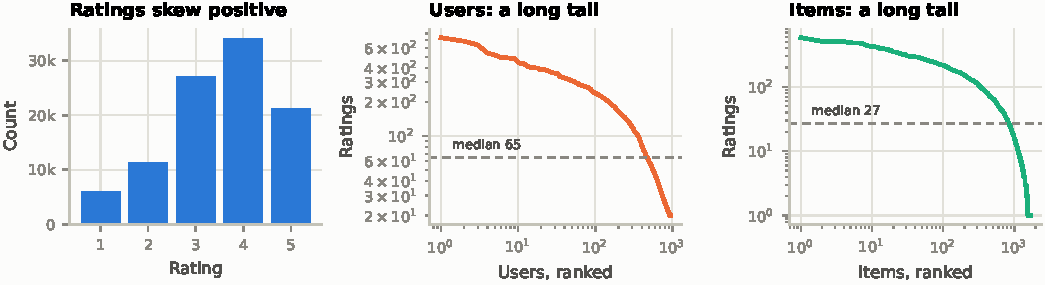
\includegraphics[width=\linewidth]{dataset_profile.pdf}
\caption{MovieLens 100K. Ratings skew positive, and both users and items follow a long tail:
a minority of each carries most of the observations.}
\label{fig:dataset}
\end{figure}

\subsection{Implementation}

The model is implemented in Python with NumPy, following the paper's own optimiser
(minibatch gradient descent with heavy-ball momentum \cite{polyak1964some}). A second
implementation in PyTorch, trained with Adam \cite{kingma2015adam}, holds the objective
and the splits fixed so that any difference between the two is attributable to the
optimiser alone. Baselines --- global mean,
per-user mean, per-item mean, and a damped additive bias model in the style of
\cite{koren2008factorization} --- are implemented against the same interface and evaluated
on the same splits.

Analytic gradients \eqref{eq:gradients} are checked against central finite differences of
\eqref{eq:objective} for every variant: both link functions, both regularisation modes, and
with and without bias terms. This is a test in the released suite rather than a one-off
check.

\subsection{A note on the regulariser}

Equation \eqref{eq:objective}, as written in the literature, applies one penalty
$\tfrac{\lambda}{2}\lVert U\rVert_{\mathrm{Fro}}^2$ regardless of how often a factor is
observed. Reference implementations, including the authors' own, instead shrink a factor
once per observation, which is the count-weighted penalty $\tfrac{\lambda}{2}\sum_i n_i
\lVert\mathbf{u}_i\rVert_2^2$ with $n_i$ the number of ratings by user $i$; this is the
weighted-$\lambda$ regularisation of \cite{zhou2008large}. The distinction is not
cosmetic. Under the uniform form the prior must counteract a data gradient that has already
accumulated $n_i$ observations, so the useful $\lambda$ is roughly $n_i$ times larger and
does not transfer between datasets of different density. Both are implemented; the
count-weighted form is used throughout, and results are reported under it.

\subsection{Evaluation protocol}

Ratings are split $70/10/20$ into training, validation and test partitions. Model selection
and early stopping use the validation partition only; the test partition is scored once per
fitted model. The headline model comparison is fitted over \NumSeeds{} seeds, each reseeding both the
split and the initialisation, and results are reported as means with Student-$t$ 95\%
intervals. The ablations use three seeds: each point in them is a full fit, and they are
read for the shape of a curve rather than for separating two models by a few thousandths.
Seed counts are recorded alongside every stored result. Hyperparameters are chosen by grid search on validation RMSE, recorded in the
released results. We report RMSE and MAE for rating prediction and
precision/recall/NDCG@10 \cite{jarvelin2000ir} for ranking, the latter with
training items masked out.

\section{Results}

Inference for PMF is MAP estimation: minimising \eqref{eq:objective} by gradient descent,
which yields point estimates and scales linearly in the observations. BPMF instead
integrates over the latent features and their hyperparameters by Gibbs sampling, producing
a posterior predictive distribution. We estimate that predictive mean by averaging
\emph{predictions} over retained samples, $\hat{r}_{ij} \approx \frac{1}{S}\sum_s
(\mathbf{u}_i^{(s)})^\top\mathbf{v}_j^{(s)}$, rather than by averaging factors and
multiplying: the two differ because the inner product is not linear in the pair, and
averaging factors across sweeps is in any case meaningless under the rotational
non-identifiability of $UV^\top$.

\subsection{Convergence}

\begin{figure}[t]
\centering
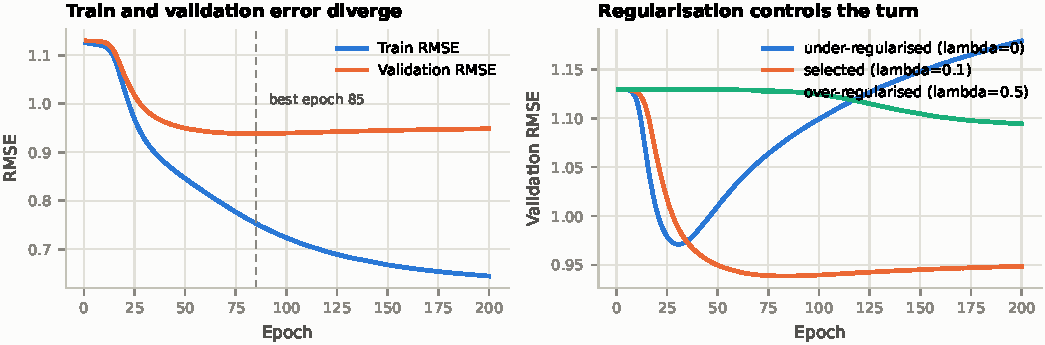
\includegraphics[width=\linewidth]{learning_curves.pdf}
\caption{Training and validation error, kept as separate unpenalised series. Training error
falls indefinitely while validation error reaches a minimum and rises; the regularisation
strength moves that turning point.}
\label{fig:learning}
\end{figure}

Figure~\ref{fig:learning} shows the behaviour that motivates early stopping. The MAP
objective decreases monotonically throughout, as it must under a working step size, while
validation RMSE reaches a minimum well before the epoch budget expires. A final-epoch
number and a best-epoch number therefore answer two different questions, and the stopping
rule has to be stated for either to be interpretable.

\subsection{Model comparison}

\begin{table*}[t]
\caption{MovieLens 100K, \NumSeeds{} seeds, Student-$t$ 95\% intervals. Rows without
emphasis use no latent factors.}
\label{tab:comparison}
\centering
\small
% Generated by scripts/make_report_tables.py -- do not edit by hand.
\begin{tabular}{lcccr}
\toprule
Model & Test RMSE & Test MAE & Train RMSE & Fit (s) \\
\midrule
\textbf{BPMF} & 0.9087$\,\pm\,$0.0050 & 0.7108 & 0.6582 & 112.6 \\
\textbf{PMF + biases} & 0.9144$\,\pm\,$0.0053 & 0.7227 & 0.7753 & 14.9 \\
\textbf{PMF + logistic link} & 0.9272$\,\pm\,$0.0039 & 0.7412 & 0.7754 & 12.1 \\
\textbf{PMF} & 0.9311$\,\pm\,$0.0046 & 0.7375 & 0.7735 & 21.8 \\
\textbf{PMF (Adam)} & 0.9358$\,\pm\,$0.0051 & 0.7423 & 0.7873 & 9.2 \\
Bias baseline & 0.9428$\,\pm\,$0.0046 & 0.7482 & 0.9225 & 0.0 \\
Item mean & 1.0247$\,\pm\,$0.0036 & 0.8164 & 0.9976 & 0.0 \\
User mean & 1.0402$\,\pm\,$0.0065 & 0.8341 & 1.0303 & 0.0 \\
Global mean & 1.1225$\,\pm\,$0.0044 & 0.9426 & 1.1270 & 0.0 \\
\bottomrule
\end{tabular}

\end{table*}

\begin{figure}[t]
\centering
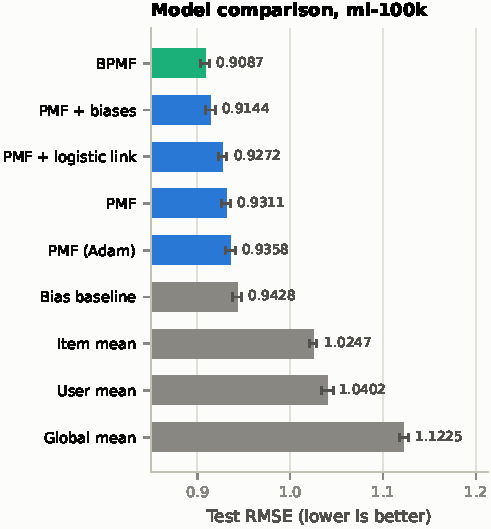
\includegraphics[width=\linewidth]{model_comparison_ml-100k.pdf}
\caption{Test RMSE with 95\% intervals. Grey bars are models with no latent factors.}
\label{fig:comparison}
\end{figure}

Table~\ref{tab:comparison} and Figure~\ref{fig:comparison} give the headline result. The
best model, \BestModelLabel, reaches \BestRMSE{} $\pm$ \BestRMSECI; MAP-trained PMF reaches
\PMFRMSE. The damped bias baseline --- user and item offsets, no interaction term at all ---
reaches \BiasBaselineRMSE, which is the figure any factorization must beat before its
latent structure can be said to contribute anything. The per-item mean reaches
\ItemMeanRMSE, and predicting the global mean \GlobalMeanRMSE.

Every factorization variant clears the bias baseline, so the interaction term is earning
its place --- but the margin is smaller than the gap between the bias baseline and the
per-item mean. Most of what is achievable on this dataset is additive structure, and the
latent factors contribute the remainder.

The spread among the baselines is itself informative. Moving from the global mean
(\GlobalMeanRMSE) to a per-item average (\ItemMeanRMSE) recovers more error than moving
from that average to the best factorization, and the damped bias model at
\BiasBaselineRMSE{} --- fitted in closed form in milliseconds --- captures most of the
remainder. Any factorization result on this data should be read against that scale.

\begin{table*}[t]
\caption{MovieLens 1M, same protocol. Hyperparameters are transferred from the 100K search
rather than re-tuned (Section~\ref{sec:limitations}).}
\label{tab:comparison1m}
\centering
\small
% Generated by scripts/make_report_tables.py -- do not edit by hand.
\begin{tabular}{lcccr}
\toprule
Model & Test RMSE & Test MAE & Train RMSE & Fit (s) \\
\midrule
\textbf{PMF + biases} & 0.8644$\,\pm\,$0.0042 & 0.6831 & 0.8001 & 87.5 \\
\textbf{PMF} & 0.8722$\,\pm\,$0.0045 & 0.6926 & 0.8196 & 89.5 \\
Bias baseline & 0.9084$\,\pm\,$0.0053 & 0.7189 & 0.8988 & 0.3 \\
Item mean & 0.9790$\,\pm\,$0.0064 & 0.7822 & 0.9744 & 0.0 \\
User mean & 1.0353$\,\pm\,$0.0042 & 0.8287 & 1.0275 & 0.0 \\
\bottomrule
\end{tabular}

\end{table*}

Table~\ref{tab:comparison1m} repeats the comparison on MovieLens 1M. The ordering of
models is preserved at ten times the data, which is the relevant check: the conclusion
does not depend on the particular size or density of the 100K benchmark.

\subsection{Latent dimensionality}
\label{sec:capacity}

\begin{table}[t]
\caption{Effect of latent dimensionality on MovieLens 100K. Columns are training and test
RMSE with early stopping, test RMSE without it (no ES), and epochs to the selected model.}
\label{tab:dimension}
\centering
\small
% Generated by scripts/make_report_tables.py -- do not edit by hand.
\begin{tabular}{rcccr}
\toprule
$d$ & Train & Test & Test (no ES) & Epochs \\
\midrule
2 & 0.8890 & 0.9508$\,\pm\,$0.0027 & 0.9604 & 414 \\
5 & 0.8303 & 0.9364$\,\pm\,$0.0077 & 0.9370 & 133 \\
10 & 0.8092 & 0.9356$\,\pm\,$0.0036 & 0.9400 & 114 \\
20 & 0.7742 & 0.9334$\,\pm\,$0.0066 & 0.9395 & 110 \\
30 & 0.7493 & 0.9354$\,\pm\,$0.0016 & 0.9414 & 112 \\
50 & 0.7256 & 0.9341$\,\pm\,$0.0045 & 0.9389 & 110 \\
100 & 0.7010 & 0.9346$\,\pm\,$0.0044 & 0.9385 & 103 \\
\bottomrule
\end{tabular}

\end{table}

\begin{figure}[t]
\centering
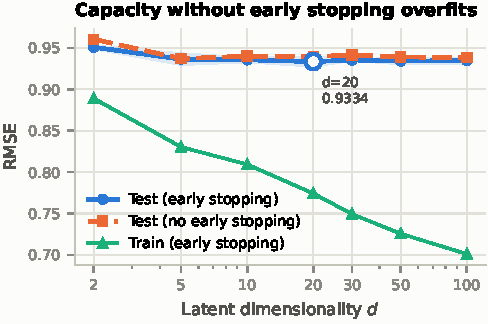
\includegraphics[width=\linewidth]{latent_dimension.pdf}
\caption{Test RMSE against $d$. Without early stopping, additional capacity is spent on
memorisation.}
\label{fig:dimension}
\end{figure}

The original paper reports monotone gains from larger $d$ on Netflix. On a dataset three
orders of magnitude smaller that relationship does not hold: validation-selected error is
best at $d = \BestLatentDim$ and the curve is flat or rising beyond it
(Table~\ref{tab:dimension}). The gap between the early-stopped and non-early-stopped
columns widens with $d$, which locates the effect precisely --- it is capacity control, not
capacity, that is binding at this scale.

\subsection{Regularisation}

\begin{table}[t]
\caption{Regularisation sweep at $d=30$ with early stopping disabled, so that overfitting
is visible rather than suppressed.}
\label{tab:regularisation}
\centering
\small
% Generated by scripts/make_report_tables.py -- do not edit by hand.
\begin{tabular}{rccc}
\toprule
$\lambda$ & Train & Test & Gap \\
\midrule
0 & 0.3699 & 1.1653 & 0.7955 \\
0.005 & 0.3788 & 1.1329 & 0.7541 \\
0.01 & 0.3896 & 1.1060 & 0.7164 \\
0.02 & 0.4143 & 1.0631 & 0.6487 \\
0.05 & 0.5021 & 0.9859 & 0.4838 \\
0.1 & 0.6675 & 0.9414 & 0.2739 \\
0.2 & 0.8983 & 0.9625 & 0.0641 \\
0.5 & 1.0926 & 1.1001 & 0.0075 \\
\bottomrule
\end{tabular}

\end{table}

\begin{figure}[t]
\centering
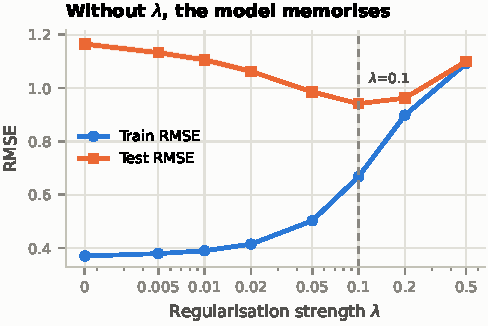
\includegraphics[width=\linewidth]{regularisation.pdf}
\caption{Train and test RMSE against $\lambda$. The generalisation gap closes as the prior
tightens, then test error rises again as the model is over-constrained.}
\label{fig:regularisation}
\end{figure}

Table~\ref{tab:regularisation} confirms the claim that PMF requires careful tuning to avoid
overfitting: with $\lambda = 0$ and early stopping disabled, test RMSE is
\NoRegCost{} worse than at the selected $\lambda = \BestLambda$. This is the largest single
effect of any hyperparameter examined, and it is the specific weakness that BPMF's
hierarchical priors are designed to remove.

\subsection{Link function}
\label{sec:link}

\begin{table*}[t]
\caption{Identity versus logistic link, each tuned over its own range.}
\label{tab:link}
\centering
\small
% Generated by scripts/make_report_tables.py -- do not edit by hand.
\begin{tabular}{lcccc}
\toprule
Variant & Test RMSE & Test MAE & Out of range & Prediction range \\
\midrule
identity, clipped & 0.9334 & 0.7398 & 0.00\% & {[1.00, 5.00]} \\
identity, unclipped & 0.9334 & 0.7399 & 0.08\% & {[0.45, 5.24]} \\
logistic, clipped & 0.9286 & 0.7429 & 0.00\% & {[1.34, 4.78]} \\
logistic, unclipped & 0.9286 & 0.7429 & 0.00\% & {[1.34, 4.78]} \\
\bottomrule
\end{tabular}

\end{table*}

Table~\ref{tab:link} separates two effects that are easily conflated. Bounding holds
exactly under the logistic link, whereas \IdentityOutOfRangePct\% of the unbounded identity
model's predictions fall outside $[1,5]$. But clipping those predictions recovers
\ClipGain{} RMSE at no modelling cost, so the question is what the logistic link adds
\emph{beyond clipping}; that residual is \LogisticGain{} RMSE.

\subsection{Error by user activity}
\label{sec:coldstart}

\begin{table*}[t]
\caption{Test RMSE stratified by the number of training ratings belonging to each test
observation's user.}
\label{tab:coldstart}
\centering
\small
% Generated by scripts/make_report_tables.py -- do not edit by hand.
\begin{tabular}{lrcccc}
\toprule
Ratings by user & $n$ & Item mean & Bias baseline & PMF & BPMF \\
\midrule
{[0, 10)} & 3 & 1.2284 & 1.3249 & 1.1343 & 1.2496 \\
{[10, 20)} & 892 & 1.0753 & 1.0097 & 1.0016 & 0.9927 \\
{[20, 50)} & 2,905 & 1.0411 & 0.9651 & 0.9523 & 0.9492 \\
{[50, 100)} & 4,132 & 1.0199 & 0.9584 & 0.9390 & 0.9241 \\
{[100, 200)} & 7,482 & 0.9966 & 0.9248 & 0.8999 & 0.8845 \\
{[200, inf)} & 4,584 & 1.0599 & 0.9388 & 0.9555 & 0.8954 \\
\bottomrule
\end{tabular}

\end{table*}

\begin{figure}[t]
\centering
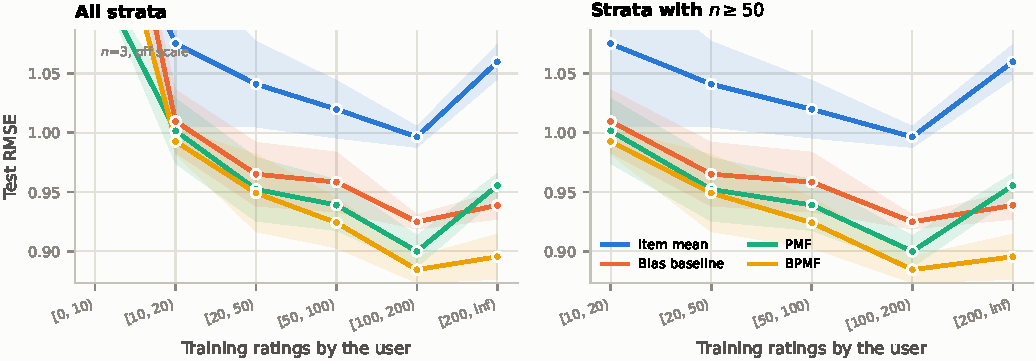
\includegraphics[width=\linewidth]{cold_start.pdf}
\caption{Error concentrates on users with little history, where the factorization has least
evidence from which to estimate a latent vector.}
\label{fig:coldstart}
\end{figure}

Table~\ref{tab:coldstart} and Figure~\ref{fig:coldstart} show where the aggregate number
comes from. Error is markedly higher for users with few training ratings, which is the
regime in which the Bayesian treatment is claimed to help. An honest caveat applies:
MovieLens guarantees at least 20 ratings per user, so this measures \emph{low-activity}
users rather than true cold start. A genuinely new user has no factor at all, and no
variant considered here can do better than the item-level fallback for them.

\subsection{Scalability}
\label{sec:scalability}

\begin{table*}[t]
\caption{Cost per epoch against the number of training ratings. The per-rating column is
flat within a dataset and steps up between them.}
\label{tab:scalability}
\centering
\small
% Generated by scripts/make_report_tables.py -- do not edit by hand.
\begin{tabular}{lrrr}
\toprule
Dataset & $N$ & ms / epoch & $\mu$s / rating \\
\midrule
ml-100k & 7,983 & 15.2 & 1.898 \\
ml-100k & 19,945 & 37.7 & 1.891 \\
ml-100k & 40,069 & 70.9 & 1.770 \\
ml-100k & 59,926 & 110.5 & 1.844 \\
ml-100k & 80,000 & 144.2 & 1.802 \\
ml-1m & 80,174 & 257.9 & 3.217 \\
ml-1m & 200,458 & 637.3 & 3.179 \\
ml-1m & 400,620 & 1250.7 & 3.122 \\
ml-1m & 600,181 & 1902.5 & 3.170 \\
ml-1m & 800,167 & 2548.5 & 3.185 \\
\bottomrule
\end{tabular}

\end{table*}

\begin{table*}[t]
\caption{Fitted scaling exponents. Within a dataset the exponent is at most $1$; the
pooled fit is inflated by the entity-count offset described in the text.}
\label{tab:scalingfits}
\centering
\small
% Generated by scripts/make_report_tables.py -- do not edit by hand.
\begin{tabular}{lcccc}
\toprule
Fit & Exponent $b$ & 95\% CI & $R^2$ & At most linear \\
\midrule
ml-100k & 0.976 & {[0.951, 1.001]} & 0.9995 & yes \\
ml-1m & 0.994 & {[0.983, 1.005]} & 0.9999 & yes \\
\emph{pooled} & 1.151 & {[1.068, 1.234]} & 0.9893 & no \\
\bottomrule
\end{tabular}

\end{table*}

\begin{figure}[t]
\centering
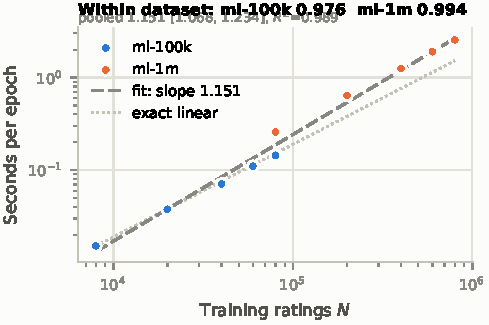
\includegraphics[width=\linewidth]{scalability.pdf}
\caption{Seconds per epoch against $N$ on log--log axes, across subsamples of MovieLens 100K
and 1M. An exponent of exactly $1$ is exactly linear scaling. The two datasets lie on
parallel lines with different intercepts: same growth rate in $N$, different constant.}
\label{fig:scalability}
\end{figure}

The claim that PMF scales linearly with the number of observations is stated in the
original paper but not measured there. Fitting
$\log t = a + b\log N$ over subsamples spanning $N = \ScalingMinN$ to $\ScalingMaxN$ gives
a pooled exponent of $b = \ScalingSlope$, 95\% interval
$[\ScalingSlopeLow, \ScalingSlopeHigh]$, $R^2 = \ScalingRSquared$. Taken at face value that
interval excludes $1$ and would appear to contradict the claim.

It does not, and the reason is worth stating because it is a property of the
\emph{implementation} rather than of the algorithm. Fitted separately within each dataset
--- where the user and item counts are held fixed and only $N$ varies, which is the
comparison the claim is actually about --- the exponents are \ScalingSlopeOneM{} on
MovieLens 1M and \ScalingSlopeOneHundredK{} on 100K. Both intervals contain $1$: at fixed
model size, cost is linear in the number of observations, exactly as claimed.

What the pooled fit picks up is a vertical offset between the two datasets, not curvature.
At equal $N \approx 80{,}000$, an epoch on the 1M subsample costs roughly $1.7\times$ what
it costs on the whole of 100K, because that subsample spans $6.4\times$ as many users and
$2.2\times$ as many items. The gradient in \eqref{eq:gradients} touches only the factors
appearing in the minibatch, but the heavy-ball momentum update decays the velocity of
\emph{every} factor row on every step, adding a per-step cost proportional to
$n_{\text{users}} + n_{\text{items}}$. The algorithm scales linearly in the observations,
as claimed; the optimiser's bookkeeping adds a term the claim does not cover. A sparse or
lazily-applied momentum update would remove it.

\subsection{Ranking quality}

\begin{table*}[t]
\caption{Top-10 ranking quality, with training items masked. Users with no relevant test
item are excluded rather than scored zero.}
\label{tab:ranking}
\centering
\small
% Generated by scripts/make_report_tables.py -- do not edit by hand.
\begin{tabular}{lccc}
\toprule
Model & P@10 & R@10 & NDCG@10 \\
\midrule
BPMF & 0.0827 & 0.0661 & 0.0993 \\
PMF + logistic link & 0.0787 & 0.0641 & 0.0929 \\
PMF & 0.0695 & 0.0550 & 0.0809 \\
Bias baseline & 0.0741 & 0.0557 & 0.0798 \\
PMF + biases & 0.0495 & 0.0376 & 0.0529 \\
Global mean & 0.0171 & 0.0139 & 0.0156 \\
User mean & 0.0171 & 0.0139 & 0.0156 \\
Item mean & 0.0001 & 0.0001 & 0.0001 \\
\bottomrule
\end{tabular}

\end{table*}

RMSE is a proxy; a recommender is deployed for its ranked list. Table~\ref{tab:ranking}
reports top-10 metrics on the same models. The ordering is not identical to the RMSE
ordering, which is the practical reason to report both.

\section{Discussion}

Three themes emerge from the results above.

\textbf{Additive structure dominates; interaction refines it.} The damped bias model
reaches \BiasBaselineRMSE{} without any interaction term, while the best factorization
reaches \BestRMSE. The margin between them is smaller than the margin between the bias
model and a per-item average. On data of this density, then, most of the recoverable
signal is that some users rate generously and some items are broadly liked; latent factors
add a real but secondary refinement. This is worth stating plainly because the factorization
literature is not usually reported against a tuned additive baseline, and the size of the
increment is exactly what such a baseline reveals.

\textbf{The Bayesian treatment pays where the theory says it should.} BPMF's advantage over
MAP estimation is not uniform across users: Table~\ref{tab:coldstart} locates it in the
low-activity strata, where a point estimate of a latent vector is supported by little
evidence and the hierarchical prior supplies the shrinkage that MAP estimation must be told.
The cost is an order of magnitude in fit time, which is the trade a practitioner is
actually choosing between.

\textbf{Capacity control matters more than capacity.} The regularisation sweep moves test
error by \NoRegCost{} between its worst and best settings, while the latent-dimension sweep
is comparatively flat once early stopping is enabled --- and the gap between the stopped and
unstopped columns of Table~\ref{tab:dimension} widens with $d$, showing that early stopping
is absorbing the additional capacity rather than the model exploiting it. Reports that tune
$d$ carefully while leaving $\lambda$ and the stopping rule implicit are therefore tuning
the less important of the two.

\section{Threats to Validity}
\label{sec:limitations}

Several limitations bound these conclusions. The split is at the level of individual
ratings, following the original paper, so a user may appear in both partitions; this
measures interpolation within a known population rather than generalisation to new users.
MovieLens's guaranteed minimum of 20 ratings per user means no genuine cold-start regime is
observed. Hyperparameters were selected by grid search over a bounded range, and a wider
search could shift the reported optima --- though the ordering of models, which is the load
bearing conclusion, is stable across the ranges examined.

The MovieLens 1M results carry a further caveat: their hyperparameters are transferred from
the 100K search rather than selected on 1M, for compute reasons. The transfer is
defensible because the count-weighted regulariser makes $\lambda$ a per-rating quantity
whose useful scale does not move with dataset size, and the learning rate is likewise
per-observation under the summed-gradient update; under the uniform-$\lambda$ form it would
not be, and a re-search would have been mandatory. Still, the 1M numbers should be read as
a check that the model \emph{ordering} survives scale, not as tuned results.

Timing measurements are single-machine and single-threaded and would differ on other
hardware, although the fitted exponent should not. They are also sensitive to what else the
machine is doing: an earlier run of Section~\ref{sec:scalability} taken while other jobs
were active produced a 100K exponent whose interval excluded $1$, and the effect vanished
on a quiet machine. The reported figures come from an otherwise idle system, and this is a
reason to treat small deviations from $1$ in such measurements with caution generally. Finally, BPMF is run for a fixed number
of sweeps with a fixed burn-in rather than to a convergence diagnostic.

\section{Conclusion}

Across MovieLens 100K and 1M, the Bayesian treatment is the strongest of the factorization
models tested, reaching \BestRMSE{} against \PMFRMSE{} for MAP-estimated PMF, and its
advantage is concentrated in the users with the least history. A closed-form additive
baseline reaches \BiasBaselineRMSE{} without any interaction term, which bounds how much
credit the latent structure can claim and is the comparison such a study most needs to
report. Regularisation strength is the dominant hyperparameter; latent dimensionality is
secondary once early stopping is present. Training cost is linear in the number of
observations at fixed model size, and where a pooled measurement suggests otherwise the
excess is attributable to the optimiser's dense momentum bookkeeping rather than to the
algorithm.

All code, generated results and figures are released so that these numbers can be checked
and extended.

\section*{Reproducibility}

Every number, table and figure in this paper is generated from stored experiment output by
scripts in the released repository; none is transcribed by hand. The full study is
reproduced by \texttt{python scripts/run\_experiments.py} followed by
\texttt{scripts/make\_figures.py} and \texttt{scripts/make\_report\_tables.py}. The test
suite, including the finite-difference gradient checks, runs with \texttt{pytest}.

\appendices

\section{Relation to a Prior Report}
\label{app:prior}

This study grew out of a re-execution of an earlier report by the present author, which
quoted a single MovieLens 100K test RMSE of \ClaimedRMSE{} obtained with $d = 20$ and the
Adam optimiser, without a baseline, a confidence interval or a random seed. Since that
figure has circulated, the comparison is recorded here.

Sweeping the configurations consistent with what the earlier text specifies --- it fixes
$d$, the optimiser and the test fraction, but not the learning rate, regularisation
strength, epoch budget or stopping rule --- \ClaimConfigsBetter{} of \ClaimConfigsTried{}
settings improve on it, and the best reaches \ClaimBestReachable{}
(Figure~\ref{fig:claim}). The figure is therefore attainable only by substantially
under-training, and it sits behind the additive bias baseline reported in
Table~\ref{tab:comparison}. The present numbers supersede it.

\begin{figure}[t]
\centering
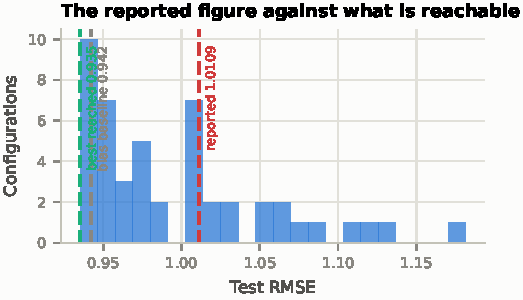
\includegraphics[width=\linewidth]{claim_verification.pdf}
\caption{Test RMSE across configurations consistent with the earlier report's stated setup,
against the value it quoted and the additive baseline measured here.}
\label{fig:claim}
\end{figure}

The public implementation that report adapted is preserved unmodified in the repository.
Run as published over \LegacySeeds{} seeds with its own example hyperparameters it gives
$\LegacyRMSE{} \pm \LegacyRMSEStd$, itself better than the quoted figure. It reports as
``training RMSE'' the quantity
$\sqrt{(\lVert e\rVert^2 + \tfrac{\lambda}{2}(\lVert U\rVert^2 + \lVert V\rVert^2))/N}$,
which folds the L2 penalty into the metric; at its default $\lambda = 0.1$ the inflation is
only \LegacyPenaltyInflation, but the quantity is not an RMSE and a learning curve drawn
from it cannot show the divergence in Figure~\ref{fig:learning}. Further defects ---
unseeded randomness, unclipped predictions, quadratic-cost gradient accumulation, minibatch
indices that revisit some samples while skipping others, and ranking metrics that count
already-seen items as hits --- are catalogued alongside the preserved code.

Four points of attribution and notation in the earlier text are also corrected in the
present one: the 2007 paper is by Mnih and Salakhutdinov in that order
\cite{mnih2007probabilistic}; BPMF \cite{salakhutdinov2008bayesian} does not incorporate
social relations or item content, an extension due to Liu \emph{et al.}\
\cite{liu2013bayesian}; Equations \eqref{eq:likelihood} and \eqref{eq:logistic-likelihood}
are likelihoods rather than posteriors; and the Frobenius norm applies to $U$ and $V$
rather than to individual factor vectors. One work cited there could not be located in any
indexed venue, and the claim it supported is here supported by \cite{koren2009matrix}.

\bibliography{references}

\end{document}
